\section{Characterization and Automated Detection of Insect Chemosensory Receptors}

\subsection{Introduction}

\subsection{Methods}

\subsubsection{Characterization}

\subsubsection{Identification Approach 1: Digrams, Weighting, and Clustering}

\subsubsection{Identification Approach 2: Profile Hidden Markov Models (HMMs)}

\subsection{Results}

\subsubsection{Characterization of Insect Chemosensory Receptors}

\begin{figure}[H]
  \centering
  \begin{subfigure}[b]{0.45\textwidth}
    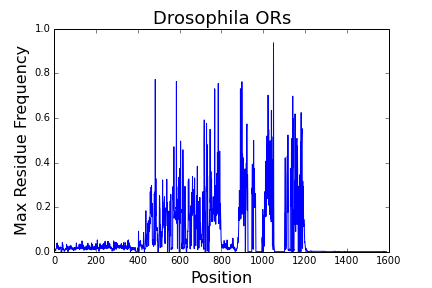
\includegraphics[width=\textwidth]{figures/chemosensory/drosophila_or_max_freq.png}
    \caption{Olfactory Receptors (930)}
    \label{fig:chemosensory:or-max-freq}
  \end{subfigure}
  ~
  \begin{subfigure}[b]{0.45\textwidth}
    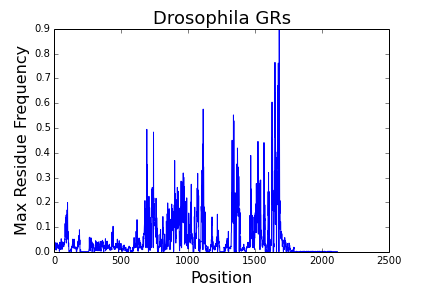
\includegraphics[width=\textwidth]{figures/chemosensory/drosophila_gr_max_freq.png}
    \caption{Gustatory Receptors (930)}
    \label{fig:chemosensory:gr-max-freq}
  \end{subfigure}
\label{fig:chemosensory:max-freq}
\caption{}
\end{figure}

\subsubsection{Comparing Approaches for Automated Identification}

\subsubsection{Identification of \emph{D. suzukii} Chemosensory Receptors}

\subsubsection{validation of \emph{D. suzukii} Chemosensory Receptors}

\subsection{Discussion and Conclusion}